% %%%%%%%%%%%%%%%%%%%%%%%%%%%%%%%%%%%%%%%%%%%%%%%%%%%%%%%%%%%%%%%%%%%%%%%%%%%%
\chapter{Dialogue modeling}%
\label{chap:modeling}
% %%%%%%%%%%%%%%%%%%%%%%%%%%%%%%%%%%%%%%%%%%%%%%%%%%%%%%%%%%%%%%%%%%%%%%%%%%%%
Modeling a dialogue is a rather complicated task.
Various architectures were proposed over the years, most of which rely on explicit data annotation on multiple levels to guide the model training process.
One of the biggest challenges is to model task-oriented dialogue that requires interaction with external interfaces s.a. databases or API services.
This aspect puts a hard constraint on the dialogue system architecture -- it requires some kind of explicit representation that allows to communicate with external systems.
It's challenging to achieve this in fully unsupervised setting, however, we explore some of the approaches in this chapter.
First, we discuss the challenges of unsupervised task-oriented dialogue modeling in more detail in Section \ref{04:to-unsup}.
Next, we propose our architecture that uses latent representations and explore its abilities and perfromance in Section \ref{04:latent-models}.
Finally, we discuss the usage of Large Language Models as dialogue models and try to answer a question if the usage of these models is able to close the gap between unsupervised and supervised systems.

\section{Task-oriented dialogue modeling with less supervision}
\label{04:to-unsup}
In this section we discuss some of the features we expect from a task-oriented dialogue and how challenging it is to implement them in an unsupervised setting.

\subsection{NLU}
\subsection{External interfaces}
Task-oriented dialogue systems must provide accurate and complete information based on user requests, which requires external database interaction.
%In order to do that, the system needs some form of external database interaction.
%
To support database access while avoiding costly turn-level annotation,
%A turn-level annotation of database queries would represent a similar amount of annotation as is used in supervised training, and thus would not lead to our desired setting, where the model is trained without labeled data.
we follow \citet{bordes2016learning} and 
insert sparse database queries and results directly into the training data, forming special dialogue turns.
Specifically, we identify turns that require database results, e.g.\ to inform about entity attributes or a number of matching entities, and insert a query-result pair in front of those turns (see Table~\ref{tab:example}).We argue that this is the minimal level of supervision required to successfully operate a task-oriented system with database access; it is significantly lower than the full dialogue-state supervision used by most systems.
In addition, it is easily available in the wild (e.g., call center transaction logs).
In practice, we observe that database queries are only inserted for 24\% turns\footnote{This is the average over all datasets in our experiments (see Section~\ref{sec:data}). Per-dataset query counts are 36\%, 23\% and 11\% for CamRest676, MultiWOZ and SMD respectively.} on average.
Note that this approach still covers the task of an explicit state tracker since the necessary entity values are provided when needed.
To maintain consistency, database query results can be stored and used in follow-up questions.

\subsection{Policy decisions}
\section{Latent Dialogue Models}
\subsection{Background}\paragraph{Variational autoencoders}
\label{04:latent-models}
\begin{figure}[t]
    \centering
    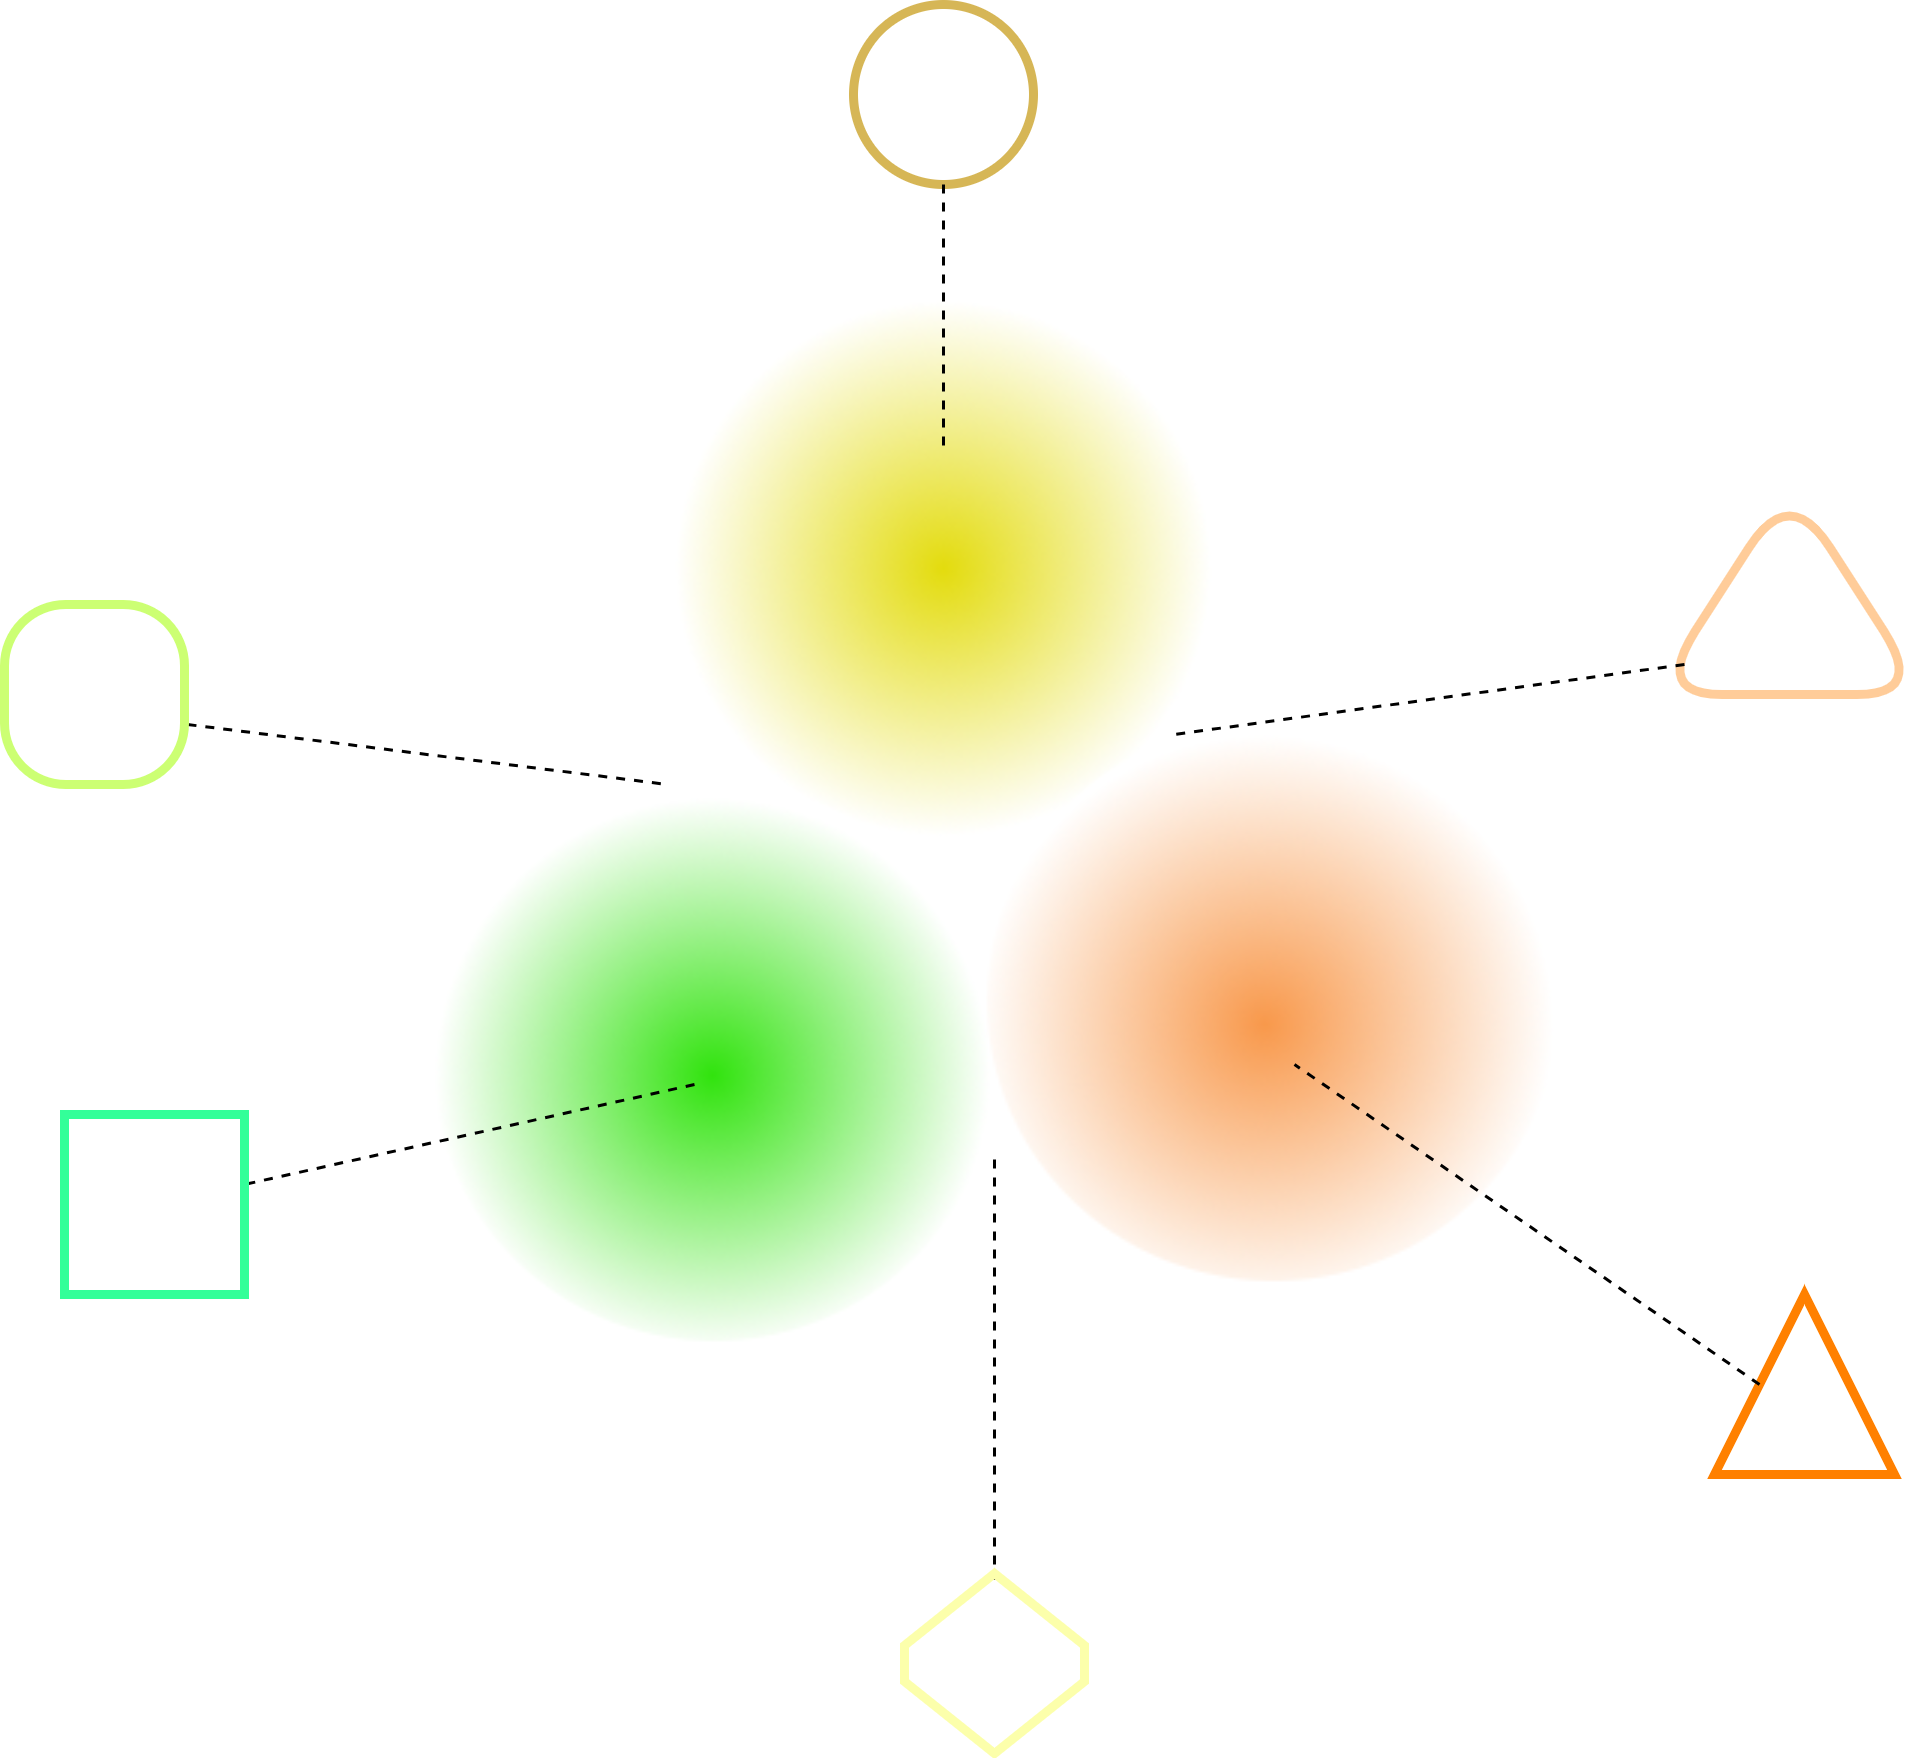
\includegraphics[width=0.46\textwidth]{images/VAE.png}
    \caption{Variational autoencoder latent space. The encoder distributions are distinguished by colors and different classes by shapes. It can be seen, the interpolation between two sampled points is meaningful}
    \label{fig:vae}
\end{figure}
Neural network training is a process during which the network learns to create internal representations of data in order to accomplish a given task.
In case of autoencoders, the task is to encode an input $\mathbf{x}$ in a way that allows for its reconstruction into the original form.
The autoencoder model consists of an encoder function $\varphi^{enc}$, which encodes an input $\mathbf{x}$ into a latent representation $\mathbf{z}$, and a decoder $\varphi^{dec}$, which models the conditional re-generation probability $p(\mathbf{x}|\mathbf{z})$.
In case of sequence autoencoders, both the encoder and decoder can be realized with an RNN.
However, vanilla autoencoders often fail to extract global semantic features of natural language sequences \cite{bowman2015generating}; therefore, adjustments need to be made in order to obtain better representations.
The technique proposed by \citet{kingma2013auto} uses the Variational Autoencoder (VAE) framework to tackle this issue.
The architecture is modified so that $\varphi^{enc}$ represents a recognition model $q(\mathbf{z}|\mathbf{x})$ which parameterizes an approximate posterior distribution over $\mathbf{z}$.
VAEs impose prior distribution on the latent variable $\mathbf{z}$, which acts as a regularization during training and makes it possible to draw samples from $q$.
Consequently, the VAE latent space is regular in a sense that it is possible to interpolate between two points.
The latent space structure is depicted schematically in Figure \ref{fig:vae}.
Typically, the modeled distributions are Gaussian and the prior is the standard normal distribution $N(0, 1)$.

We can realize the function modules in VAE using neural networks, however, there is a drawback regarding the implementation of sampling.
The sampling operation is not differentiable and therefore cannot be trained using standard approaches.
A solution to this problem is to use the \textit{reparameterization trick} \cite{kingma2013auto}.
The reparameterization trick uses the fact that a random variable under certain conditional distribution can be expressed as a deterministic transformation of some other variable with independent marginal distribution.
Distributions that allow us to do such a transformation include \textit{Gaussian, Logistic} or \textit{Gumbel}.

\paragraph{VAE latent space discretization}
Although VAE training yields robust representations that are also more interpretable thanks to the regularized latent space, in some cases, we require the latent representations to be discrete.
The motivation is mainly to improve interpretability and possibly uncover underlying processes in sequential tasks.
It is problematic to incorporate discrete variables into neural network models, because the widely used backpropagation algorithm requires smooth differentiable functions in order to propagate the gradients correctly.
\citet{van2017neural} propose a vector quantization technique to discretize the latent variables in VAEs.
Another approach is to use the the Gumbel-softmax distribution \cite{jang2016categorical} that enables us together with the reparameterization trick (Section \ref{sec:vae}) to work with categorical variables while not breaking the gradient flow in the network.

\paragraph{Variational Recurrent Neural Networks}
\label{sec:vrnn}
Variational Recurrent Neural Networks (VRNN) \cite{chung2015recurrent} explicitly model the dependencies between latent random variables across subsequent timesteps, similarly to dynamic Bayesian networks such as Hidden Markov Models (HMMs).
Unlike HMMs, the transitions between latent states are dependent not only on the state in the current time step, but also on the RNN hidden state which allows to model more complex dynamics.
Therefore, VRNNs are well suited for modeling sequential processes.
Basically, the VRNN is a recurrent network with a VAE in every time step.
The difference with respect to a basic VAE is that both prior and posterior distributions as well as the decoder are dependent on the RNN hidden state.
Formally, let $\mathbf{h}_{t}$ be the RNN hidden state in time step $t$.
The prior is realized with function $\varphi^{prior}(\mathbf{h}_{t-1})$, the posterior distribution $q$ is modeled with $\varphi^{enc}(\mathbf{x}_t, \mathbf{h}_{t-1})$ and the generation decoder distribution is $\varphi^{dec}(\mathbf{z}_t, \mathbf{h}_{t-1})$.

\section{Pretrained Language Models}
\subsection{\todo{}}
\begin{itemize}
    \item AuGPT - other experiments - using only portion of train set; compute number of training iterations; compare to RNNs
    \item LLM experiments
    \item Put it all together? is our NLU method able to improve performance of ZS LLMs/ latent models?
    \item Make work https://github.com/HLTCHKUST/Mem2Seq and look at the copy distributions
\end{itemize}